\chapter{Adversarial Constructions: How Lower Bounds Get Built}

An upper bound is a promise; an impossibility result is the proof that no better promise exists. The second kind of theorem is not derived from the first --- it is \emph{built}. To show that no algorithm, language, or sketch in a model can do better, the author must construct the world in which every allowable procedure fails: a pair of instances, a hard distribution, a stream of updates engineered so that succeeding is impossible and failing is provable. That engineered world is the \emph{adversary}, the workhorse of impossibility. In our corpus the tool is used by 21 of 228 tagged papers, and it owns the survey's signature pairing: 13 of those papers prove an upper bound \emph{and} its matching adversarial lower bound in the same article. The pairing is no accident --- the upper bound tells you what the adversary must force; the adversary certifies that the upper bound is the end of the line.

\section{The Tool: Anatomy of an Adversarial Argument}

Strip away the domain vocabulary and adversarial arguments share a three-part skeleton.

\paragraph{The world: an instance family.}
Fix the model of computation or observation --- the rows of a linear sketch, a stream of tuple inserts and deletes, the syntax of an algebra, a class of colored graphs. Inside that model, design the instance family: often two planted instances $I_0$ and $I_1$, or, via Yao's minimax principle~\cite{adversarial-construction-bg1}, a single hard input distribution against which the best deterministic procedure is analyzed.

\paragraph{Forced behavior or information blindness.}
Argue that \emph{every} procedure in the model is constrained on the family, for one of two reasons. \emph{Information blindness}: the observation available to the algorithm (a sketch, a transcript, a vector of walk counts) simply does not contain the bit that distinguishes the instances. \emph{Forced behavior}: the model's own syntax caps a resource --- e.g.\ an expression of size $\ell$ can multiply tuple multiplicities by at most $2^{\ell}$ --- and the adversary exhibits an instance whose correct answer exceeds every cap.

\paragraph{The two-instance indistinguishability pattern.}
The decisive move: instances $I_0$ and $I_1$ produce identical observations yet demand different answers, so any output is wrong on one of them.

\begin{center}
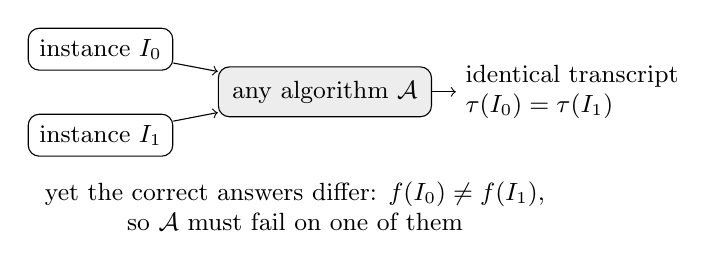
\begin{tikzpicture}[scale=0.95, every node/.style={font=\small}]
  \node[draw, rounded corners, inner sep=4pt] (I0) at (0,1.15) {instance $I_0$};
  \node[draw, rounded corners, inner sep=4pt] (I1) at (0,0) {instance $I_1$};
  \node[draw, rounded corners, inner sep=5pt, fill=black!7] (A) at (3,0.58) {any algorithm $\mathcal{A}$};
  \node[align=left, anchor=west] (T) at (4.75,0.58) {identical transcript\\$\tau(I_0)=\tau(I_1)$};
  \draw[->] (I0) -- (A);
  \draw[->] (I1) -- (A);
  \draw[->] (A) -- (T);
  \node[align=center] at (2.6,-0.95) {yet the correct answers differ: $f(I_0)\neq f(I_1)$,\\ so $\mathcal{A}$ must fail on one of them};
\end{tikzpicture}
\end{center}

\paragraph{Imported adversaries: reductions and communication complexity.}
When no direct planting suffices, the adversary is imported. A conditional lower bound is an adversary-as-reduction: an effective procedure converts instances of a believed-hard problem ($k$-clique, OuMv, SETH) into instances or update sequences of yours, so any fast algorithm would refute the conjecture --- the dominant pattern for dynamic graph and query problems~\cite{adversarial-construction-bg5}. Communication complexity hands out prefabricated two-player adversaries --- index, set-disjointness, gap-Hamming --- whose transcripts are information-blind by construction~\cite{adversarial-construction-bg2}; sketching lower bounds in databases have ridden this route since the frequency-moment bound~\cite{adversarial-construction-bg3}. And when the object under attack is a \emph{language} rather than a cost, the adversary is a witness object, from Moon--Moser's triangle graph~\cite{adversarial-construction-bg4} to the counterexamples that have measured relational completeness since Codd~\cite{adversarial-construction-bg6}.

\section{Exemplars from the Corpus}

\subsection{Walk-Equivalent Graph Pairs and GNN Expressiveness}

MPLang is a matrix-programming language capturing GNN-style computation over embedded graphs; its affine fragment A-MPLang omits activation functions. What can the affine fragment even see?

\begin{corollary}
The following are equivalent for pointed $d$-embedded graphs $(G_1,\gamma_1,v_1)$ and $(G_2,\gamma_2,v_2)$:
\begin{enumerate}
  \item $e(G_1,\gamma_1)(v_1) = e(G_2,\gamma_2)(v_2)$ for every A-MPLang expression $e$ of $A^{+}$-depth $n$ over $d$-embeddings;
  \item $((A^{+})^{i}\,1)(G_1,\gamma_1)(v_1) = ((A^{+})^{i}\,1)(G_2,\gamma_2)(v_2)$ and $((A^{+})^{i}P_j)(G_1,\gamma_1)(v_1) = ((A^{+})^{i}P_j)(G_2,\gamma_2)(v_2)$ for all $i \in [n]$ and $j \in [d]$.
\end{enumerate}
The condition in the second item defines $(G_1,v_1,\gamma_1)$ and $(G_2,v_2,\gamma_2)$ being \emph{$n$-walk equivalent}.
\end{corollary}

A normal-form theorem shows every affine expression of depth $n$ is a fixed polynomial in the walk-count features of item 2, so any two graphs agreeing on those counts are indistinguishable to the entire fragment --- the textbook two-instance pattern, with walk statistics as the shared transcript. A single walk-equivalent pair that disagrees on the target query kills the fragment, and red--blue symmetric trees (with induction on expression shape) extend the witnessing to separate activation-function classes: any $\Sigma$-MPLang expression must stay symmetric exactly where a ReLU threshold can break symmetry. \cite{sigmod26-004}\pods{}

\subsection{Sketching Dimension for $\ell_2$ Sampling}

A linear $\ell_2$-sampling sketch observes $Sv$ and must output coordinate $i$ with probability roughly $v_i^2/\lVert v\rVert_2^2$. How many rows must $S$ have, and how many bits store $Sv$?

\begin{theorem}
An $(\epsilon,\delta)$-$\ell_2$-sampler with frequency estimation requires a sketching dimension of at least $\Omega\bigl(\tfrac{1}{\epsilon}\log^2 n + \tfrac{2}{\epsilon}\log n\bigr)$. Moreover, storing such a sketch for vectors with poly$(n)$-sized entries requires $\Omega\bigl((\log^3 n + \tfrac{2}{\epsilon}\log^2 n)/\epsilon\bigr)$ bits.
\end{theorem}

The adversary is a planted distribution made rigorous by Yao's principle: $m$ short Gaussian spikes sit on isotropic background noise, so each row of the sketch observes a location mixture $X \sim N(v_I, I_d)$ with $I$ uniform and $\lVert v_i\rVert \le 10\ln m$. The paper's Lemma 2 bounds recovery of $I$ from $X$ by $2m^{-1/2}$ --- the spikes are information-blind to any decoder --- and a payout-game argument converts failed identification into sampling error. \cite{sigmod26-241}\pods{}

\subsection{Conditional Lower Bounds for Dynamic Query Maintenance}

A dynamic algorithm maintains the answers to a fixed conjunctive query $Q$ under single-tuple inserts and deletes, with amortized update time and enumeration delay. Which maintenance times are achievable without blowing up the update cost?

\begin{theorem}
Assuming the combinatorial $k$-clique conjecture, no dynamic combinatorial algorithm can maintain $Q$ with amortized update time $O(|D|^{(k-1)/k-\epsilon})$ and support constant-delay enumeration, for any constant $\epsilon > 0$.
\end{theorem}

Here the adversary is imported: a reduction encodes $k$-cycle detection (via color-coding hash families) and OuMv tensor products into an update sequence on the database, so a faster maintenance algorithm would solve the conjecture-hard problem. The reduction \emph{is} the adversary --- it generates the stream adaptively, and indistinguishability is inherited from the source problem rather than planted directly. \cite{sigmod26-244}\pods{}

\subsection{Expressiveness: Relational Algebra Without Division}

On $\mathbb{K}$-databases every tuple carries a semiring value, and the paper asks which fragments of calculus and algebra still coincide in the spirit of Codd's theorem~\cite{adversarial-construction-bg6}. One operation resists every expression.

\begin{theorem}
There is no expression of basic relational algebra $\mathrm{BRA}$ that defines the division operation $\div$ on $\mathbb{N}$-databases.
\end{theorem}

This is forced behavior by a counting ceiling: structural induction shows every $\mathrm{BRA}$ expression $E$ on inputs of size $n$ has support at most $n^{\ell(E)}$ and multiplicities at most $p_E(n)\cdot 2^{\ell(E)}$ --- single-exponential growth in expression size. The adversary is one $2^n$-multiplicity division instance, which outruns the budget of every fixed expression; no pair of instances is needed, only growth rates. \cite{sigmod26-290}

\subsection{Output-Sensitive Witness Graphs for Defective Cliques}

A $k$-defective clique is a vertex set missing at most $k$ edges; enumeration algorithms are judged by search space relative to output. How large must the output itself be in the worst case?

\begin{theorem}
The worst-case output size of maximal $k$-defective clique enumeration is $\Omega(3^{n/3}\cdot n^{k})$ when $k$ is a constant.
\end{theorem}

The adversary is a Moon--Moser-style witness graph~\cite{adversarial-construction-bg4}: disjoint triangles already force an independent three-way choice per block ($3^{n/3}$ maximal cliques), and each of the $k$ units of permitted defect contributes another polynomial factor of choices. The construction bounds \emph{every} enumeration algorithm --- the output itself is that large --- and thereby certifies the paper's worst-case-optimal search space as tight. \cite{sigmod26-306}

\begin{reachbox}{When to Build an Adversary}
\begin{itemize}
  \item You have (or plan) an upper bound and need to certify optimality: aim the adversary at exactly the resource your algorithm touches --- this is the 13-paper pairing, not a coincidence.
  \item The question is ``can \emph{any} method in this model do better'' or ``is this language expressive enough'', not ``is my implementation correct''.
  \item Recipe: fix the observation model; find what all procedures must share (a transcript, a growth ceiling, a symmetry); plant two instances that share it but demand different answers; or import the pair from a conjecture-hard problem via a reduction, or from communication complexity.
  \item Against randomized algorithms, invoke Yao's principle first and design a hard \emph{distribution}; the analysis then runs against deterministic procedures.
  \item If every two-instance attempt fails, take the hint: perhaps the model is sufficient. Try the matching upper bound before fighting the lower bound.
\end{itemize}
\end{reachbox}
